\documentclass[11pt]{article}
\usepackage[usenames,dvipsnames]{pstricks}
\usepackage{epsfig}
\usepackage{pst-grad} % For gradients
\usepackage{pst-plot} % For axes
\usepackage[space]{grffile} % For spaces in paths
\usepackage{etoolbox} % For spaces in paths
\usepackage{graphicx}
\definecolor{light-gray}{gray}{0.95}
\makeatletter % For spaces in paths
\patchcmd\Gread@eps{\@inputcheck#1 }{\@inputcheck"#1"\relax}{}{}
\makeatother

\usepackage{xcolor}
\usepackage{dsfont}
\setlength{\oddsidemargin}{.25in}
\setlength{\evensidemargin}{.25in} \setlength{\textwidth}{6in}
\setlength{\topmargin}{-0.4in} \setlength{\textheight}{8.5in}
\def\argmax{\mathop{\rm arg\,max}}

\usepackage{xspace,epsfig,amsmath,amssymb,subfig,lmodern}

\newtheorem{theorem}{Theorem}
\newtheorem{lemma}{Lemma}
\newtheorem{definition}{Definition}
\newtheorem{corollary}{Corollary}
\newcommand{\B}{\mathcal{B}}
\newcommand{\A}{\mathcal{A}}
\newcommand{\N}{\mathcal{N}}
\renewcommand{\S}{\mathcal{S}}

\newenvironment{sketch}{\noindent\emph{Proof Sketch:}}{$\quad \Box$}
\newenvironment{proof}{\noindent\emph{Proof:}}{$\quad \Box$}
\newcommand{\handout}[5]{
   \renewcommand{\thepage}{\arabic{page}}
   \noindent
   \begin{center}
   \framebox{
      \vbox{
    \hbox to 5.78in { {\bf Choice Models in Operations}  \hfill #2
}
       \vspace{4mm}
       \hbox to 5.78in { {\Large \hfill #5  \hfill} }
       \vspace{2mm}
       \hbox to 5.78in { {\it #3 \hfill #4} }
      }
   }
   \end{center}
   \vspace*{4mm}
}

\begin{document}

\handout{}{}{Instructor: Srikanth Jagabathula}
{Scribe:  Katherine Hoffmann } {Lecture 
  2  :  Utility Theory}


\begin{definition}
A preference relation $\succcurlyeq$ is said to be represented by a \underline{utility function} \\
$u: \N \rightarrow \mathbb{R}$ if and only if $$ x \succcurlyeq y \iff u(x) \geq u(y)$$
\end{definition}

{\color{gray}Utility functions map preference relations over items in the universe to an ordered relation defined over real numbers. At this point, we haven't required that $\succcurlyeq$ is a rational preference relation; we also haven't required that such a function actually exists.}
\\

If a utility function exists, it induces a choice rule defined as:
$$ C(\B, u(\cdot))  =\{x \in \B ~|~ x \text{ is a solution of }\max_{y \in \B} u(y)\}$$

{\color{gray} When can a preference relation be represented by a utility function? 
 It appears that rationality is necessary for the existence of a utility function $\ldots$ Is it sufficient?}

\begin{theorem}
If $\N$ is finite, then any complete and transitive preference relation can be represented by a utility function $u:\N\rightarrow\mathbb{R}$.
\end{theorem}
\begin{sketch}
Proof by induction (recursive approach). 
Suppose $|\N| = n$; then, we can construct a mapping from $\N$ to $\{1, 2, \ldots, n\}$. 
Consider $C(\N; \succcurlyeq)$, the set of most preferred elements in $\N$. Since $C$ is a choice function induced by weak preference, this set is nonempty. Now, take all of the elements in $C(\N; \succcurlyeq)$ and map them to $n$. Remove to obtain $\N^* = \N \setminus C(\N; \succcurlyeq)$, and repeat the same steps on $\N^*$, assigning the value $n-1$ to the most preferred elements in $\N^*$. Repeat until there are no elements left.
\end{sketch}

~

{\color{gray}
So, finiteness and rationality are sufficient to guarantee the existence of a utility function to represent the preference relation $\succcurlyeq$.

$$C(\cdot)\xrightarrow{\text{HARP}}\text{  rational choice rule  }\xrightarrow[\text{of $\N$}]{\text{finiteness }}\text{  utility representation  }$$
}

 \fcolorbox{gray}{white}{
\begin{minipage}{0.9\textwidth} 
{\color{gray}
\underline{Example.} Given a choice rule $C$, how can we determine whether it is rational?
Suppose $C (\cdot)$ is a singleton (univalent). Given revealed preferences for a collection of sets $\B_1, \B_2, \B_3$, and in particular supposing $C(\B_i)=x_i, ~\forall ~1 \leq i \leq m$, we can answer this question algorithmically with a graph representation. 
\begin{enumerate}
\item We can portray revealed preferences on a directed graph $G$, with the elements of $\N$ as nodes and a directed edge $(x,y)$ if there exists $\B_i$ such that $(x,y) \in \B_i$ and $y \in C(\B_i)$. 
\item If the graph has a directed cycle, transitivity is violated (we can check this with the Floyd-Warshall Algorithm). 
\item If the graph is not complete, we can extend it by assuming indifference between elements or ranking elements (if transitivity holds, at least one such extension exists).
\end{enumerate}}
\end{minipage}}

~

{\color{gray}
Next, we introduce the idea of probabilistic or stochastic choice. Why? 
\begin{enumerate}
	\item Relax the rationality assumption. For example, suppose there exists a set of items $\{a,b\}$ for which a consumer sometimes likes $a$ and sometimes likes $b$. We can model the consumer as drawing from a distribution of preferences, where the consumer's preferences are only rational within the span of a given day.
	\item Model choices of populations. For example, if $a$ is chosen 10 times and $b$ is chosen 10 times, we can model a set of 20 people with heterogeneous preferences.
\end{enumerate}}
To proceed, we assume that $\N$ is finite, and in each choice instance, only one element is chosen.

\begin{definition}
A \underline{stochastic choice rule} is specified as $\mathbb{P}(\cdot | \cdot)$, where $\mathbb{P}(x|\B)$ denotes the probability that $x$ is chosen from $\B$. 
\end{definition}
We assume that $\mathbb{P}(\cdot|\cdot)$ satisfies the usual probability rules:
\[\begin{array}{llll}
	1. & 0 \leq \mathbb{P}(x|\B) \leq 1, & \forall x \in \B, ~\forall B  & \text{(Probabilities between 0 and 1)} \\ [6pt]
	2. & \sum_{x \in \B} \mathbb{P}(x|\B) = 1, & \forall B& \text{(Normalization condition)} \\ [6pt]
	3. & \mathbb{P}(x \text{ or }y|\B) = \mathbb{P}(x|\B) + P(y|\B) && \text{(Only one item chosen)} \\
	& \mathbb{P}(x \text{ and }y | \B) = 0
\end{array}\]

Remark: Deterministic choice rules are a special case of stochastic choice rules as defined here. 

{\color{gray} To capture a deterministic univalent rational choice rule, it is sufficient to have one preference order (a.k.a. preference list, rank list, permutation). To capture a stochastic choice rule, the order is not sufficient.}

\begin{definition}
A stochastic choice rule $\mathbb{P}(\cdot | \cdot)$ is \underline{stochastically rational} if there exists a probability measure $\pi$ on $\S_n$ such that:
$$P(x|\B) = \pi(\succ \in \S_n: x = \succ \B)$$
where either $x \succ y \in \B,~\forall~ y \neq x$, or $x$ is the unique $\succ$-maximal element in $\B$. Here, $x=\succ \B$ means ``$x$ is the most preferred element in set $\B$'', and $\S_n$ is the set of all possible linear (complete, transitive, and antisymmetric) preference relations $\succ$  on the set $\N$. 
\end{definition}

 \fcolorbox{gray}{white}{
\begin{minipage}{0.9\textwidth} 

{\color{gray}
\underline{Example.} Let $\N = \{x,y,z\}$. Suppose:
\[\begin{array}{rclcrcl}
\mathbb{P}(x|\{x,y\}) &=& \frac{3}{4} && \mathbb{P}(y|\{x,y\}) &=& \frac{1}{4}
\end{array}\]

Is this stochastically rational? To answer this question, we need to construct a probability mass over all possible preference orderings:
\[\begin{array}{clcclccl}
x \succ y \succ z & (\sigma_1) && y \succ x \succ  z &(\sigma_3)&& z \succ x \succ y & (\sigma_5) \\
x \succ z \succ y & (\sigma_2) && y \succ z \succ  x &(\sigma_4)&& z \succ y \succ x &(\sigma_6) \\
\end{array}\]
Then, we have:
$$ Pr(x \text{ chosen from } \B \text{ under probability distribution } \pi) = \pi(\sigma_1) + \pi(\sigma_2) + \pi(\sigma_5) $$ 
So, for example, we could have:
\[\begin{array}{rclcrclcrcl}
\pi(\sigma_1) &=& \frac{3}{4}  &~~~& \pi(\sigma_3) &=& \frac{1}{4} &~~~& \pi(\sigma_i) &=& 0 \text{ otherwise }
\end{array}\]}
\end{minipage}}

~\\~

Remark: Not every stochastic choice rule is stochastically rational.

~

\fcolorbox{gray}{white}{
\begin{minipage}{0.9\textwidth} 
{\color{gray}
\underline{Example.} Let $\N = \{x,y,z\}$. Suppose:
\[\begin{array}{rclcrcl}
\mathbb{P}(x| \{x,y\}) &=& \frac{3}{4} && \mathbb{P}(y| \{x,y\}) &=& \frac{1}{4} \\ [6pt]
\mathbb{P}(y| \{y, z\}) &=& \frac{3}{4} && \mathbb{P}(z| \{y,z\}) &=& \frac{1}{4} \\ [6pt]
\mathbb{P}(z| \{x, z\}) &=& \frac{3}{4} && \mathbb{P}(x| \{x,z\}) &=& \frac{1}{4} \\
\end{array}\]

This is unsolvable. These probabilities imply that $\mathbb{P}(x \text{ is chosen from }\{x,z\}) \geq \frac{1}{2}$, which is a contradiction.}

~

\centerline{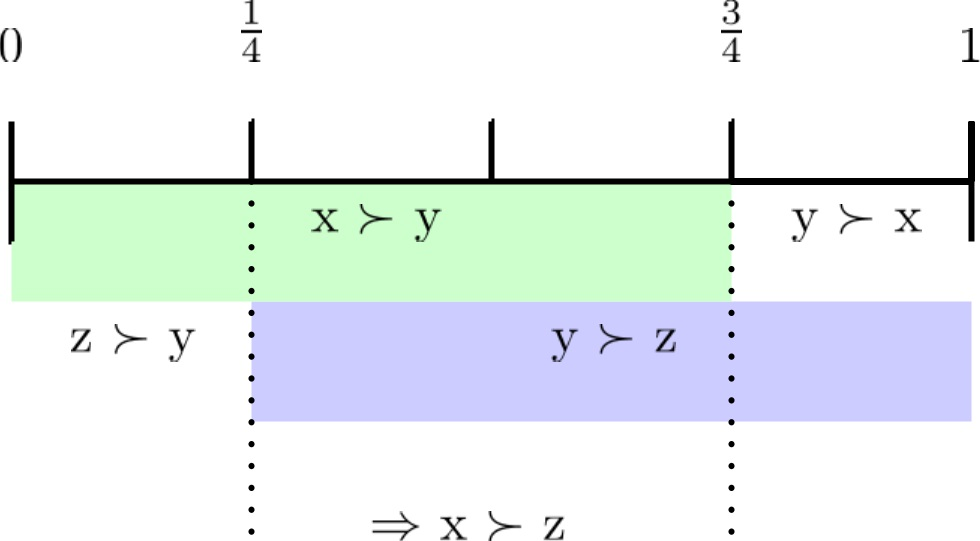
\includegraphics[width=3in]{figures/choice_figure.jpg}}

~

\end{minipage}}


~

 {\color{gray} So, under what conditions is a rule stochastically rational? Such conditions exist, but they are hard to verify.}

\begin{definition}
\underline{Axiom of Revealed Stochastic Preference (ARSP).} A stochastic choice rule $\mathbb{P}(\cdot|\cdot)$ defined over $\N$ satisfies ARSP if, for every finite collection of tuples $(x_1, \B_1), (x_2, \B_2), \ldots, $ $(x_n, \B_n)$ such that $x_i \in \B_i, ~\forall~ i$, we have that:
$$\sum^m_{i=1} k_i ~\mathbb{P}(x_i | \B_i) ~~\leq~~ \max_{\succ \in \S_n} ~ \sum^m_{i=1} k_i ~\mathds{1}[\succ, x_i, \B_i]$$
for any collection of nonnegative integers $k_i, i=1,\ldots, m$ and where 
$$\mathds{1}[\succ, x, \B] = \begin{cases}1 & \text{if }x \in C(\B) \\ 0 & \text{otherwise} \end{cases}$$
\end{definition}

% \psscalebox{1.0 1.0} % Change this value to rescale the drawing.

% \begin{pspicture}(0,-1.805)(6.535,1.805)
% \definecolor{colour0}{rgb}{0.8,0.8,1.0}
% \definecolor{colour1}{rgb}{0.8,1.0,0.8}
% \psframe[linecolor=colour0, linewidth=0.04, fillstyle=solid,fillcolor=colour0, dimen=outer](6.475,-0.205)(1.675,-1.005)
% \psframe[linecolor=colour1, linewidth=0.04, fillstyle=solid,fillcolor=colour1, dimen=outer](4.875,0.595)(0.075,-0.205)
% \psline[linecolor=black, linewidth=0.04](6.475,0.595)(6.475,0.995)(6.475,0.195)
% \psline[linecolor=black, linewidth=0.04](0.075,0.595)(6.475,0.595)(4.875,0.595)
% \psline[linecolor=black, linewidth=0.04](0.075,0.995)(0.075,0.195)(0.075,0.195)
% \psline[linecolor=black, linewidth=0.04](1.675,0.995)(1.675,0.995)(1.675,0.595)
% \psline[linecolor=black, linewidth=0.04](4.875,0.995)(4.875,0.995)(4.875,0.595)
% \rput[b](4.875,1.395){$\frac{3}{4}$}
% \rput[b](1.675,1.395){$\frac{1}{4}$}
% \rput[b](0.075,1.395){0}
% \rput[b](6.475,1.395){1}
% \rput[bl](3.675,-0.605){y $\succ$ z}
% \rput[bl](0.475,-0.605){z $\succ$ y}
% \rput[bl](2.075,0.195){x $\succ$ y}
% \rput[bl](5.275,0.195){y $\succ$ x}
% \psline[linecolor=black, linewidth=0.04](3.275,0.995)(3.275,0.995)(3.275,0.595)
% \psline[linecolor=black, linewidth=0.04, linestyle=dotted, dotsep=0.10583334cm](1.675,0.595)(1.675,-0.605)(1.675,-1.805)
% \psline[linecolor=black, linewidth=0.04, linestyle=dotted, dotsep=0.10583334cm](4.875,0.595)(4.875,0.595)(4.875,-1.805)
% \rput[bl](2.475,-1.805){$\Rightarrow$ x $\succ$ z}
% \end{pspicture}


\begin{theorem}
A stochastic choice rule $\mathbb{P}(\cdot | \cdot)$ is stochastically rationalizable iff it satisfies ARSP.
\end{theorem}
\end{document}
